\chapter{Elektromagnetiese stra\-ling}\fancyfoot[LO,RE]{Fisika: Golwe, Klank en Lig}
    \setcounter{figure}{1}
    \setcounter{subfigure}{1}
    \label{459e2bef85baf867f5850bc8338cad3a}
         \section{Wat is \textsl{elektromagnetiese straling}?}
    \nopagebreak
Die eerste voorbeeld van elektromagnetiese (e\-lek\-tro\-mag\-ne\-tie\-se) straling is lig. Almal is vertroud met lig in die alledaagse lewe, en mens kan voorwerpe slegs sien wanneer lig daarvan af weerkaats en jou oog binnedring. Hierdie enkele eienskap van lig maak dit betekenisvol genoeg om van lig te leer. Daar is egter ook baie ander toepassings van e\-lek\-tro\-mag\-ne\-tie\-se straling. Dit word elektromagneties genoem, want daar is elektriese en magnetiese velde wat saam die straling opmaak. Ons sal hierdie konsep bietjie later in meer diepte ondersoek. 

\chapterstartvideo{VPefg}

Alhoewel lig in die alledaagse lewe nie baie ooglopende spesiale eienskappe blyk te h\^e nie, moet mens tog let op die volgende: 
\begin{itemize}
 \item \textbf{'n Wye spektrum}: Die lig wat ons kan sien (sigbare e\-lek\-tro\-mag\-ne\-tie\-se straling) is slegs 'n klein deel van die bestaande e\-lek\-tro\-mag\-ne\-tie\-se stralingsspektrum. 
 \item \textbf{Die natuur se spoedgrens}: Niks beweeg vinniger as die spoed van lig nie.  
 \item \textbf{Golfgeaardheid}: Alle e\-lek\-tro\-mag\-ne\-tie\-se straling het die vermo\"e om op te tree soos 'n golf. 
 \item \textbf{Partikel geaardheid}: Alle e\-lek\-tro\-mag\-ne\-tie\-se straling het die vermo\"e om op te tree soos 'n partikel.
 \item \textbf{Geen medium benodig}: e\-lek\-tro\-mag\-ne\-tie\-se straling kan voortplant sonder die teenwoordigheid van 'n medium waardeur dit beweeg, selfs al het dit 'n golfgeaardheid.
\end{itemize}

Twee belangrike konsepte om van kennis te dra, soos hierbo genoem:
\begin{enumerate}[noitemsep, label=\textbf{\arabic*}. ]
 \item golfgeaardheid sonder 'n nodige medium om in te beweeg, en 
 \item beide 'n partikel en 'n golf. 
\end{enumerate}
Ons sal die bogenoemde in die volgende afdelings bespreek, en in selfs meer detail in Graad 11 en 12 ingaan. 

    \label{m38777*cid3}
            \section{Golfaard van e\-lek\-tro\-mag\-ne\-tie\-se straling}
            \nopagebreak
      \label{m38777*id186686}As jy kyk na 'n klomp miere wat loop van een punt na 'n ander, dan lyk dit na 'n dun ononderbroke swart lyn. Maar as jy egter die lyn miere van nader bekyk, sal jy sien dat die lyn miere bestaan uit duisende afsonderlike miere.\par 
      \label{m38777*id187029}Lig en alle ander tipes elektromagnetiese straling blyk ook 'n ononderbroke golf aanvanklik te wees, maar wanneer mens eksperimente met lig uitvoer, begin 'n mens agterkom dat lig beide golf sowel as partikel eienskappe het. Net soos die individuele miere, bestaan die lig ook uit individuele bundels energie, of kwanta van lig.\par 
     
 \label{m38777*id187035}Lig het beide golf en deeltjie (partikel) eienskappe (golf-partikel dualiteit of dubbelaard), maar slegs die een of die ander word getoon, afhangende van die aard van die eksperiment wat uitegevoer word. 'n Golf-tipe eksperiment toon die golf natuur, en 'n partikel-tipe eksperiment toon die partikel natuur. 'n Mens kan nie die golf en die partikel geaardheid op dieselfde tydstip toets nie. 'n Ligpartikel staan bekend as 'n foton.\par 




\Definition{Foton}{ 'n Foton is 'n kwantum (energiepakkie) lig.} 



\subsection*{Velde}
            \nopagebreak
      \label{m38777*id187125}\textit{Versnellende ladings} straal elektromagnetiese golwe uit. 'n Veranderende elektriese veld wek 'n magnetiese veld op en 'n veranderende magnetiese veld word wek 'n elektriese veld op. Hierdie is die onderliggende beginsel by die voorplanting van elektromagnetiese golwe, aangesien elektromagnetiese golwe, anders as klankgolwe, nie 'n medium benodig om deur te beweeg nie.  

\mindsetvid{Animation of electric fields}{VPeka}

E\-lek\-tro\-mag\-ne\-tie\-se golwe plant voort wanneer 'n elektriese veld, ossillerend op een vlak, 'n magnetiese veld veroorsaak wat op een vlak ossilleer teen 'n 90 grade hoek daarmee, wat dan weer 'n ossillerende magnetiese veld veroorsaak, ensovoorts.   Die voorplanting van die elektromagnetiese golwe kan beskyf word as \textsl{wedersydse induksie}.\par Ons gebruik $E$ om elektriese velde aan te dui, en $B$ om magnetiese velde aan te dui\par

Hierdie wedersydse opwekkende velde beweeg deur 'n vakuum teen 'n konstante spoed van $3\ensuremath{\times}{10}^{8}\phantom{\rule{0.166667em}{0ex}}\text{m}\ensuremath{\cdot}{\text{s}}^{-1}$, voorgestel deur $c$.\par 
      \label{m38777*eip-43}Alhoewel 'n elektromagnetiese golf deur 'n vakuum kan beweeg, kan dit ook deur 'n medium soos water en lug beweeg. Wanneer 'n elektromagnetiese golf egter deur 'n medium beweeg, sal dit stadiger beweeg as wanneer dit deur 'n vakuum sou beweeg.\par \label{m38777*id187191}
    \setcounter{subfigure}{0}
	\begin{figure}[H] % horizontal\label{m38777*id187194}
    \begin{center}

\begin{pspicture}(-4,-4)(3,4)
\psset{Alpha=30}
\pstThreeDCoor[nameY=$B$,nameZ=$E$,linecolor=black,xMin=-4,yMin=-4,zMin=-4]
\parametricplotThreeD[xPlotpoints=200,linecolor=blue,linewidth=1.5pt,plotstyle=curve,linestyle=dashed](-180,180){%
    t 60 div
    3 2.5 t mul cos mul
    0}
\parametricplotThreeD[xPlotpoints=200,linecolor=red,linewidth=1.5pt,plotstyle=curve](-180,180){%
    t 60 div
    0
     -3 2.5 t mul cos mul
    }
\end{pspicture}
\caption{
 'n Diagram wat die wedersydse opwekkende (aanhoudend skeppende) elektriese veld (soliede rooi lyn) en magnetiese veld (blou stippeltyn) aandui.
}

 \end{center}
 \end{figure}       
      \par \label{m38777*eip-808}Aangesien e\-lek\-tro\-mag\-ne\-tie\-se straling 'n golf is, sal die volgende formula steeds van toepassing wees: \par \label{m38777*eip-181}\nopagebreak\noindent{}
    \begin{equation*}
    v=f\ensuremath{\cdot}\lambda
      \end{equation*}
      \label{m38777*eip-601}Behalwe dat ons ons $v$ kan vervang met $c$:\par \label{m38777*eip-194}\nopagebreak\noindent{}
    \begin{equation*}
    \boxed{c=f\ensuremath{\cdot}\lambda}
      \end{equation*}
      \par


\begin{wex}{E\-lek\-tro\-mag\-ne\-tie\-se straling I}{
Bereken die frekwensie van 'n elektromagnetiese golf met 'n golflengte van $4,2\ensuremath{\times}{10}^{-7}$ m.}
{ 
\westep{Golfvergelyking}
Ons gebruik die vergelyking: $c=f\lambda $ om frekwensie te bepaal. Die spoed van lig is konstant $3\ensuremath{\times}{10}^{8}$m/s.\par 

\westep{Bereken}  
\begin{equation}
    \begin{array}{ccl}\hfill c& =& f\lambda \hfill \\ \hfill 3\ensuremath{\times}{10}^{8}& =& f\ensuremath{\times}4,2\ensuremath{\times}{10}^{-7}\hfill \\ \hfill f& =& 7,14\ensuremath{\times}{10}^{14}\text{Hz}\hfill \end{array}
\end{equation}


\westep{Skryf die finale antwoord neer}

Die frekwensie is $7,14\times10^{14}$Hz.

}
\end{wex}
 
\begin{wex}{E\-lek\-tro\-mag\-ne\-tie\-se Bestraling II}{
'n Elektromagnetiese golf het 'n golflengte van $200\phantom{\rule{3.33333pt}{0ex}}\text{nm}$. Wat is die frekwensie van die straling?}{

\westep{Wat weet ons?}
Onthou dat alle straling beweeg teen die spoed van lig ($c$) in 'n vakuum.
Aangesien die vraag nie spesifiek aandui deur watter materie die golf beweeg nie, is dit veilig vir ons om te aanvaar dat die golf beweeg deur 'n vakuum. 
Ons kan twee eienskapp van die straling identifiseer - golflengte $\phantom{\rule{3.33333pt}{0ex}}\left(200\phantom{\rule{3.33333pt}{0ex}}\text{nm}\right)$ en spoed ($c$).\par 

\westep{Pas die golfvergelyking toe} 
\begin{equation}
    \begin{array}{ccc}\hfill c& =& f\lambda \hfill \\ \hfill 3\ensuremath{\times}{10}^{8}& =& f\ensuremath{\times}200\ensuremath{\times}{10}^{-9}\hfill \\ \hfill f& =& 1.5\ensuremath{\times}{10}^{15}\phantom{\rule{4pt}{0ex}}\text{Hz}\hfill \end{array}
\end{equation}

\westep{Skryf die finale antwoord neer}

Die frekwensie is $1,5\times10^{15}$Hz.
}
\end{wex}

\section{Elektromagnetiese spektrum}
            \nopagebreak
e\-lek\-tro\-mag\-ne\-tie\-se straling word geklassifiseer in tipes, afhangend van die frekwensie van die golf: hierdie tipes sluit in, in volgende van toenemendheid van die frekwensie, radiogolwe, mikrogolwe, infrarooi straling, sigbare lig, ultraviolet straling, x-strale en gammastrale. \par 
            \nopagebreak
      
            \mindsetvid{Electromagnetic spectrum}{VPemp}


      \label{m38778*id187332}Table \ref{table:EMSpectrumRanges} Lys die golflengte en frekwensie reeks van die afdeldings van die elektromagnetiese sprektrum.\par 
    % \textbf{m38778*uid8}\par
          \begin{table}[H]
    % \begin{table}[H]
    % \\ '' '0'
        \begin{center}
      \label{m38778*uid8}
    \noindent
    
      \begin{tabular}[t]{|l|l|l|}\hline
                \textbf{Kategorie}
               &
                \textbf{Golflengtegebied(nm)}
               &
                \textbf{Frekwensiegebied(Hz)}
              % make-rowspan-placeholders
     \tabularnewline\cline{1-1}\cline{2-2}\cline{3-3}
      %--------------------------------------------------------------------
        gammastrale &
        $\lessthan{}$1 &
                $\greatthan{}3\ensuremath{\times}{10}^{19}$
              % make-rowspan-placeholders
     \tabularnewline\cline{1-1}\cline{2-2}\cline{3-3}
      %--------------------------------------------------------------------
        X-strale &
        1-10 &
        $3\ensuremath{\times}{10}^{17}$-$3\ensuremath{\times}{10}^{19}$% make-rowspan-placeholders
     \tabularnewline\cline{1-1}\cline{2-2}\cline{3-3}
      %--------------------------------------------------------------------
        ultraviolet lig &
        10-400 &
        $7,5\ensuremath{\times}{10}^{14}$-$3\ensuremath{\times}{10}^{17}$% make-rowspan-placeholders
     \tabularnewline\cline{1-1}\cline{2-2}\cline{3-3}
      %--------------------------------------------------------------------
        sigbare lig &
        400-700 &
        $4,3\ensuremath{\times}{10}^{14}$-$7,5\ensuremath{\times}{10}^{14}$% make-rowspan-placeholders
     \tabularnewline\cline{1-1}\cline{2-2}\cline{3-3}
      %--------------------------------------------------------------------
        infrarooi &
        700-${10}^{5}$ &
        $3\ensuremath{\times}{10}^{12}$-$4,3\ensuremath{\times}{10}^{19}$% make-rowspan-placeholders
     \tabularnewline\cline{1-1}\cline{2-2}\cline{3-3}
      %--------------------------------------------------------------------
        mikrogolf &
                ${10}^{5}-{10}^{8}$
               &
        $3\ensuremath{\times}{10}^{9}$-$3\ensuremath{\times}{10}^{12}$% make-rowspan-placeholders
     \tabularnewline\cline{1-1}\cline{2-2}\cline{3-3}
      %--------------------------------------------------------------------
        radiogolwe &
                $\greatthan{}{10}^{8}$
               &
                $\lessthan{}3\ensuremath{\times}{10}^{9}$
              % make-rowspan-placeholders
     \tabularnewline\cline{1-1}\cline{2-2}\cline{3-3}
      %--------------------------------------------------------------------
    \end{tabular}
      \end{center}
    \caption{Elektromagnetiese spektrum}
    \label{table:EMSpectrumRanges}
\end{table}
    \par
      \label{m38778*id188548} Voorbeelde van sommige gebruike van elektromagnetiese golwe word gewys in Tabel \ref{table:EMUses}.\par 

\begin{table}[H]
    \begin{center}
    \begin{tabular}{|l|m{10cm}|}\hline
    \textbf{Kategorie}
    &
    \textbf{Gebruike} \\ \hline
    gammastrale &
    gebruik om die bakterie in malvalekkers dood te maak, sowel as vir die sterilisasie van mediese toerusting \\ \hline
    
    X-strale &
    gebruik om beenstrukture grafies voor te stel \\ \hline
    
    ultraviolet lig &
    bye kan ultraviolet lig sien, omdat blomme meer uitstaan by hierdie frekwensie.\\ \hline
    sigbare lig &
    word gebruik deur mense om die wereld te bekyk en bestudeer \\ \hline
    infrarooi &
    nagvisie, hittesensors, laser metaalsnywerk \\ \hline 
    mikrogolf &
    mikrogolfoonde, radar \\ \hline 
    radiogolwe &
    radio, televisieuitsendings\\ \hline
    \end{tabular}
    \end{center}
\caption{Gebruike van e\-lek\-tro\-mag\-ne\-tie\-se golwe}
\label{table:EMUses}
\end{table}


\begin{exercises}{}{
\begin{enumerate}[noitemsep, label=\textbf{\arabic*}. ] 
    \item Rangskik die volgende tipes e\-lek\-tro\-mag\-ne\-tie\-se straling in volgorde van toenemende frekwensie: infrarooi, x-strale, ultraviolet, sigbare lig en gammastrale.\newline
    \item Bereken die frekwensie van 'n e\-lek\-tro\-mag\-ne\-tie\-se golf met 'n golflengte van 400~nm.\newline
    \item Gee 'n voorbeeld van die gebruike van elke tipe e\-lek\-tro\-mag\-ne\-tie\-se straling, bv. gammastrale, X-strale, ultraviolet ligstrale, sigbare lig, infrarooi, mikrogolwe en radio- en televisiegolwe.\newline
\end{enumerate}
\label{m38778*cid6}
\practiceinfo
 \par \begin{tabular}[h]{cccccc}
 (1.) 028a  &  (2.) 028b  &  (3.) 028c  & \end{tabular}
}\end{exercises}

\begin{figure}[H] % horizontal\label{m38778*uid3}
\begin{center}
\rule[.1in]{\figurerulewidth}{.005in} \\
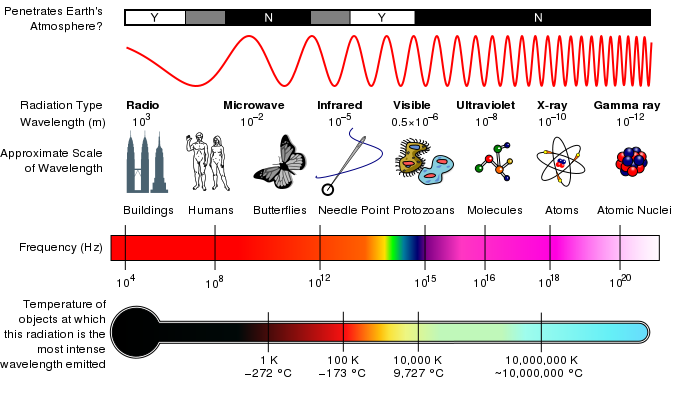
\includegraphics[width=\columnwidth]{col11305.imgs/m38778_EM_Spectrum_Properties_edit.png} % m38778;e\-lek\-tro\-mag\-ne\-tie\-se\_Spectrum\_Properties\_edit.png;;;6.0;8.5;
\caption{Die elektromagnetiese spektrum as a funksie van frekwensie. Die verskillende tipes afhangend van golflengte  sowel as alledaagse vergelykings word gewys.}
\label{fig:emspectrum}
\rule[.1in]{\figurerulewidth}{.005in} \\
\end{center}
\end{figure}       


\label{m38778*id187230}E\-lek\-tro\-mag\-ne\-tie\-se straling in die sigbare deel van die spektrum word deur alle voorwerpe rondom ons verstrooi. Die elektromagnetiese straling verskaf inligting aan ons o\"e wat ons toelaat om te kan sien. Die frekwensies straling waarvoor die menslike oog sensitief is, is slegs 'n baie klein deel van al die moontlike frekwensies van e\-lek\-tro\-mag\-ne\-tie\-se straling. Die volle stel van e\-lek\-tro\-mag\-ne\-tie\-se straling word genoem die elektromagnetiese sprektrum. Om die konsep te vereenvoudig, word die sprektrum verdeel in onderafdelings, naamlik radio, mikrogolf, infrarooi, sigbare lig, ultraviolet lig, x-strale en gammastrale. \par
 
\label{m38778*eip-855}Die e\-lek\-tro\-mag\-ne\-tie\-se spektrum is aaneenhoudend (sonder gapings) en oneindig. Weens tegnologiese beperkings, kan ons slegs elektromagnetiese straling gebruik met golflengtes tussen ${10}^{-14}\text{m}$ en ${10}^{15}\text{m}$.
           

\section{Deurdringingsvermo\"e van elektromagnetiese straling}
\nopagebreak
Verskillende frekwensies van e\-lek\-tro\-mag\-ne\-tie\-se straling het verskillende deurdringingsvermo\"e. Byvoorbeeld, as ons die menslike liggaam as objek gebruik, dan word sigbare lig gereflekteer van die oppervlak van die menslike liggaam af, ultraviolet lig (van die son) beskadig die vel, maar x-strale kan die vel en been penetreer en maak foto's van binne die menslike liggaam moontlik. \par 

As ons die energie van sigbare lig vergelyk met die energie van x-strale, dan vind ons dat x-strale het 'n veel ho\"er frekwensie. Gewoonlik het elektromagnetiese straling met 'n ho\"er frekwensie 'n ho\"er penetrasie vermo\"e as die met laer frekwensies. \par 

Sommige tipes elektromagnetiese straling soos ultraviolet strale, x-strale en gammastrale is baie gevaarlik. Bestraling afkomstig van hierdie tipes staan bekend as ioniserende straling. Ioniserende straling dra energie oor soos dit deur materie beweeg, breek molekulere verbindings af en skep ione. \par 

Oormatige blootstelling aan straling, insluitende sonlig, x-strale en alle kernkrag straling, kan die ontbinding van biologiese weefsel veroorsaak. Gelukkig beskerm die aarde se atmosfeer ons en ander lewende wesens van meeste van die skadelike e\-lek\-tro\-mag\-ne\-tie\-se straling..\par 

            \subsubsection*{Ultraviolet (UV) straling en die vel}
            \nopagebreak
        \label{m38779*id189482} UVA en UVB is verskillende reekse van frekwensies van (UV) lig. UVA en UVB kan kollageen vesels beskadig wat dan die resultaat het van verhoogde vel veroudering. Oor die algemeen is UVA die minder skadelike een van die twee, alhoewel dit bydra tot die veroudering van vel, DNA skade en moontlike vel kanker. Dit dring deur op 'n diep vlak, en veroorsaak nie sonbrand nie. \par 
        \label{m38779*id189490}UVB lig kan velkanker veroorsaak. Die straling affekteer die DNA molekule in die vel se selle, wat dan kan veroorsaak in moontlike kankeragtige mutasies. Die osoonlaag in die atmosfeer beskerm ons teen UVB straling. Die verhouding tussen UVB straling en kanker is een van die redes vir kommer rakende die afname van osoon in die atmosfeer. \par 
        
\label{m38779*id189495}Die menslike liggaam raak bruin wanneer dit bootgestel word aan 'n matige (afhangend van vel tipe) vlak van straling, deur die vrystel van die bruin pigment melanin. Dit help om om UV deurdringing te blok, en voorkom skade aan die meer sensitiewe vel weefsel. Sonbrandolie blok UV straling gedeeltelik en is geredelik beskikbaar. Hierdie produkte het 'n sonbeskermingsfaktor (SBF) aanduiding (gewoonlik aangedui op die houer) wat aandui tot watter mate die produk beskerming bied teen UVB straling. Die SBF dui nie aan wat die beskerming is teen UVA straling nie. Sommige sonbrand-olie bevat deesdae titanium dioksied wat kan help beskerm teen UVA straling. Ander UVA afwerende stowwe gevind in sonbrand-olie sluit in sink dioksied en avobenzone. \par 
\label{m38779*secfhsst!!!underscore!!!id701}
\begin{minipage}{.5\textwidth}
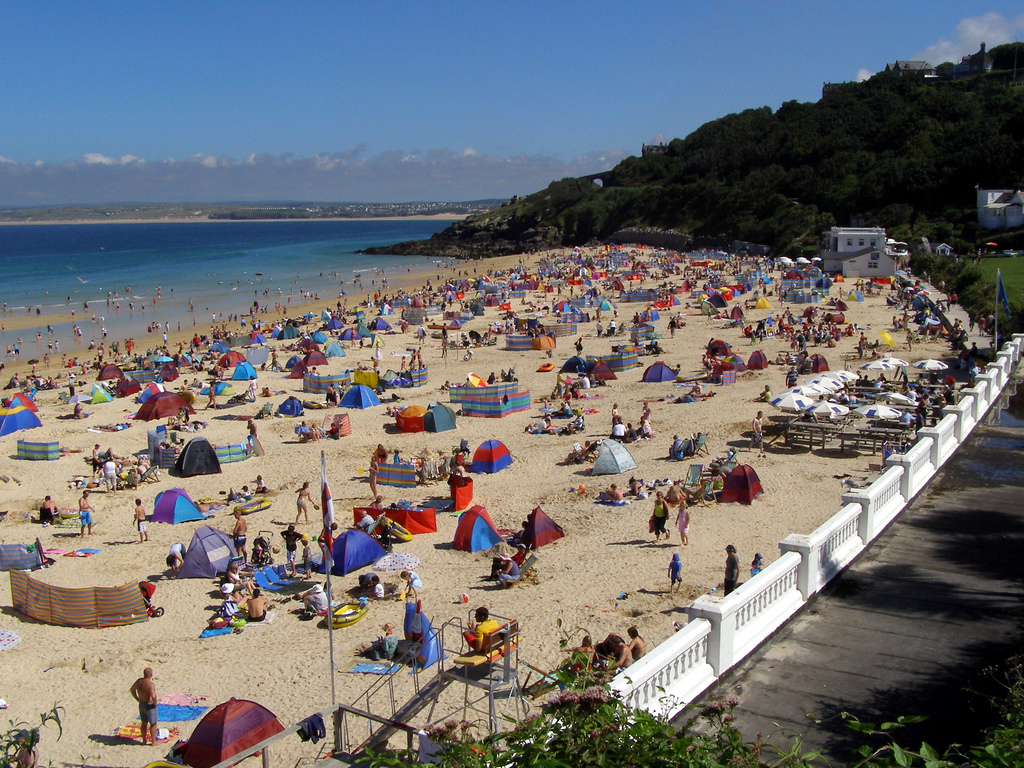
\includegraphics[width=.8\columnwidth]{photos/beach2_treehouse1977.jpg}
\end{minipage}
\begin{minipage}{.5\textwidth}
            \subsubsection*{Wanneer is sonbrandolie effektief?}
            \nopagebreak
        \label{m38779*id189518}\begin{itemize}[noitemsep]
            \label{m38779*uid18}\item UVB beskerming: Padimate O, Homosalate, Octisalate (octyl salicylate), Octinoxate (octyl methoxycinnamate)
\label{m38779*uid19}\item UVA beskerming: Avobenzone
\label{m38779*uid20}\item UVA/UVB beskerming: Octocrylene, titanium dioksied, sink oksied, Mexoryl (ecamsule)
\end{itemize}
        \label{m38779*id189561} 'n Verdere manier om UV te blok, is deur die dra van spesifieke klere wat beskerm teen die son. Dit is klere wat 'n UPF gradering het wat die beskerming teen beide UVA en UVB beskryf. \par 
      \label{m38779*uid21}
\end{minipage}
            \subsubsection*{Ultraviolet straling en die o\"e}
            \nopagebreak
        \label{m38779*id189581}Hoe intensiteit UVB lig kan skade veroorsaak aan die o\"e, en blootstelling kan foto keratitis ("arc eye") veroorsaak, en kan lei tot katarakte en ander mediese toestande. \par 
        \label{m38779*id189586}Beskermende oogtoestelle is voordelig vir diegene wat werk met of blootgestel is ultraviolet straling. Gegewe dat die lig die oog kan bereik ook van die kante, is volle oogbeskerm aanbeveelbaar. 
        \label{m38779*id189594} Gewone, onbehandelde brille bied ook tot 'n mate beskerming. Plastiek lense bied meer beskerming as glas lense. Sommige plastiese lens materiale soos poliekarbonaat, blokkeer die meeste UV strale. Meeste kontaklense beskerm die retina deur die absorbsie van UV straling. \par 
      \label{m38779*uid22}
      \begin{minipage}{.5\textwidth}
            \subsubsection*{X-strale}
            \nopagebreak
        \label{m38779*id189613}Alhoewel x-strale gebruik word in die mediese veld, kan verlengde blootstelling aan x-strale lei tot sel skade en kanker. \par 
        \label{m38779*id189617} Byvoorbeeld, 'n mammogram is 'n x-straal van die menslike bors om borskanker te vind, maar indien 'n vrou op 'n gereelde basis mammogramme ontvang terwyl sy te jonk is, verhoog haar kanse om borskanker op te doen. \par 
      \label{m38779*uid23}
            \subsubsection*{Gammastrale}
            \nopagebreak
        \label{m38779*id189632}As gevolg van die hoe energie vlakke van gammastrale, kan hierdie strale ernstige skade veroorsaak wanneer dit geabsorbeer word deur lewende selle. \par 
        \label{m38779*id189636}Gamma-strale word nie gestop deur die vel nie, en kan DNA verandering tot gevolg h\^e deur inmenging met die genetiese materiaal van die sel. DNA "dubbele band" breke word oor die algemeen aanvaar as die mees biologies betekenisvolle letsel te wees wat deur ioniserende straling kanker en oorerflike siekte bevorder. \par 
        \label{m38779*id189642} 'n Studie gedoen op Russiese kernkragwerkers wat blootgestel was aan uitwendige volle-liggaam gamma-bestraling teen ho\"e dossise wys 'n verband tussen blootstelling aan die straling en sterftes gekoppel aan bloedkanker, sowel as long-, lewer-, skeletale en ander vaste kankers. \par 
      \label{m38779*eip-665}
\end{minipage}
\begin{minipage}{.5\textwidth}\begin{center}
 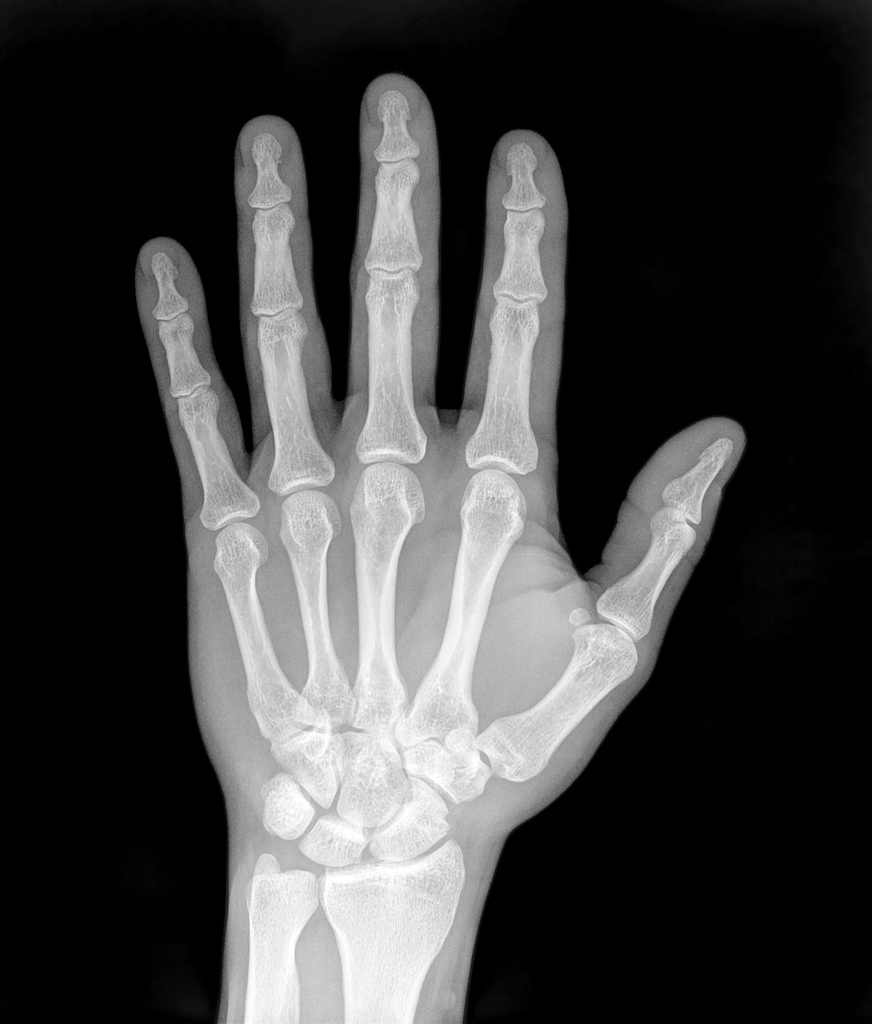
\includegraphics[width=0.8\textwidth]{photos/x-ray-hand_TraceMeek_flickr.jpg}\end{center}
\end{minipage}

            \subsubsection*{Selfone en mikrogolfbestraling}
            \nopagebreak
\begin{minipage}{.5\textwidth}
\includegraphics[width=.8\columnwidth]{photos/cellphones_kapungo.jpg}
\end{minipage}
\begin{minipage}{.5\textwidth}
            \label{m38779*id189654} Selfoon straling en gesondheids kwessies is al geopper, veral weens die enorme verhoging in selfoongebruik. Die rede agter die kommer is omdat selfone gebruik maak van elektromagnetiese golwe in die mikrogolfreeks. Hierdie kwessies het al gelei tot 'n groot volume navorsing. Kommer oor die effek op gesondheid is ook al geopper rakende ander draadlose digitale stelsels, soos datakommunikasie netwerke. 
In 2009 het die Wereld Gesondheidsorganisasie aangekondig dat hulle 'n verband gevind het tussen breinkanker en selfone. Daar is egter nog nie konkrete bewyse vir hierdie stelling nie, en die verband is meestal vaag. Jy kan meer uitvind by: http://www.who.int/mediacentre/factsheets/fs193/en/\footnote{http://www.who.int/mediacentre/factsheets/fs193/en/}
        \par 
\end{minipage}
        \label{m38779*id189664} Selfoongebruikers word aangeraai om hul blootstelling aan straling te minimaliseer, deur byvoorbeeld:\par 
        \label{m38779*id189668}\begin{enumerate}[noitemsep, label=\textbf{\arabic*}. ] 
            \label{m38779*uid24}\item Die gebruik van 'n handvrye toestel ("hands-free") om die straling na die brein te laat afneem.
\label{m38779*uid25}\item Hou die selfoon weg van jou liggaam.
\label{m38779*uid26}\item Moenie 'n selfoon in 'n motor gebruik sonder 'n eksterne antenna nie. 
\end{enumerate}
        \label{m38779*uid27}
            \begin{exercises}{Deurdringingsvermo\"e van e\-lek\-tro\-mag\-ne\-tie\-se straling}
            \nopagebreak
        \label{m38779*id189729}\begin{enumerate}[noitemsep, label=\textbf{\arabic*}. ] 
            \label{m38779*uid28}\item Dui aan die deurdringingsvermo\"e van die verskillende tipes e\-lek\-tro\-mag\-ne\-tie\-se straling en koppel dit aan die energie wat verband hou met die uitstraling. \newline
\label{m38779*uid29}\item Beskryf die gevare van gammastrale, x-strale en die skadelike effek van ultaviolet straling op jou vel. \newline
\end{enumerate}
    \label{m38779*cid8}
\practiceinfo
 \par \begin{tabular}[h]{cccccc}
 (1.) 028d  &  (2.) 028e  & \end{tabular}
\end{exercises}


            \section{Die partikelaard van elektromagnetiese straling}
            \nopagebreak
      \label{m38778*id188832} Wanneer ons praat van elektromagnetiese straling as 'n partikeldeeltjie, dan verwys ons na fotone, wat pakkies energie is. Die energie van die foton hou verband met die golflengte van die elektromagnetiese straling volgens:\par 
\label{m38778*fhsst!!!underscore!!!id476}\Definition{Planck se konstante}{\label{m38778*meaningfhsst!!!underscore!!!id476}
      \label{m38778*id188843}Planck se konstante is 'n fisiese konstante vernoem na Max Planck.\par 
      \label{m38778*id188849}$h=6,626\ensuremath{\times}{10}^{-34}$ J $\ensuremath{\cdot}$ s
 \par 
       } 
      \label{m38778*id188898} Die energie van 'n foton kan bereken word met die gebruik van die volgende formule: $E=hf$ or $E=h\frac{c}{\lambda }$.
Waar E die energie van die foton in joules is (J), h is Planck se konstante, c is die spoed van lig, f is die frekwensie in hertz (Hz) en $\lambda $ is die golflengte in meters (m).\par Hoe ho\"er die frekwensie van die e\-lek\-tro\-mag\-ne\-tie\-se straling is, hoe ho\"er is die energie gekoppel daaraan.  
\begin{wex}
{Die berekening van die energie van 'n foton I
}
{
Bereken die energie van 'n foton met 'n frekwensie van $3\ensuremath{\times}{10}^{18}$~Hz}
{
\westep{Ontleed die probleem.}
Jy is gevra om die energie van 'n foton te bepaal. Die frekwensie is in standaardeenhede en jy ken die verwantskap tussen frekwensie en energie.

\westep{Pas die formule toe vir die energie van 'n foton.}
\begin{eqnarray*}
E& =& hf\\ 
& =& 6,6\ensuremath{\times}{10}^{-34}\ensuremath{\times}3\ensuremath{\times}{10}^{18}\\ 
& =& 2\ensuremath{\times}{10}^{-15}\phantom{\rule{0.166667em}{0ex}}\text{J}
\end{eqnarray*}

\westep{Skryf die finale antwoord neer.}
die energie us $2\times10^{-15}$ J
}
\end{wex}
    
\begin{wex}{Die berekening van die energie van 'n foton II}{Wat is die energie van 'n ultraviolet foton met 'n golflengte van 200~nm?}{
\westep{Ontleed die probleem.}
Jy is gevra om die energie van 'n foton waarvan die golflengte gegee is, te bepaal. Die golflengte is in standaard eenhede en jy ken die verwantskap tussen frekwensie en energie. Ons weet ook wat die verwantskap tussen golflengte en frekwensie is, die golfspoedvergelyking. Die spoed van lig is 'n bekende konstante.

\westep{Pas die beginsels toe.}
Eerstens bepaal ons die frekwensie in terme van golflengte.
\begin{eqnarray*}
c &=& f\cdot\lambda\\
f &=& \frac{c}{\lambda}
\end{eqnarray*}
Ons vervang dit in die vergelyking vir die energie van 'n foton. 
\begin{eqnarray*}
E&=& h \cdot f\\
& =& h\frac{c}{\lambda }\hfill \\ 
& =& \left(6,626\ensuremath{\times}{10}^{-34}\right)\frac{3\ensuremath{\times}{10}^{8}}{200\ensuremath{\times}{10}^{-9}}\hfill \\ 
& =& 9,939\ensuremath{\times}{10}^{-10}\phantom{\rule{0.166667em}{0ex}}\text{J}
\end{eqnarray*}

\westep{Skryf die finale antwoord neer.}
Die energie van die foton is $9,939\times10^{-10}$ J.
}
\end{wex}

\begin{exercises}{Partikel aard van e\-lek\-tro\-mag\-ne\-tie\-se golwe}
\begin{enumerate}[noitemsep, label=\textbf{\arabic*}. ]
    \item Wat is die verband tussen die energie van 'n foton met die frekwensie en die golflengte van die foton? \newline
    \item Bepaal die energie van 'n foton (e\-lek\-tro\-mag\-ne\-tie\-se straling) met 'n frekwensie van ${10}^{12}$~Hz.\newline
    \item Bepaal die energie van 'n foton (e\-lek\-tro\-mag\-ne\-tie\-se straling) met 'n golflengte van 600 nm.\newline
\end{enumerate}
  \label{m38778**end}
\practiceinfo
 \par \begin{tabular}[h]{cccccc}
 (1.) 028f  &  (2.) 028g  &  (3.) 028h  & \end{tabular}
\end{exercises}
            
\label{m38779*eip-745}
\subsection*{Gedrag van Diere}
\nopagebreak
Mense glo al vir eeue dat diere kan aanvoel wanneer 'n aardbewing of ander natuurramp op hande is. Reeds in 373 V.C, het historici al opgeteken rakende massiewe uittogte van diere, insluitende rotte, slange en meerkatte wat uit die Griekse stad Helice gevlug het voordat dit deur 'n aardbewing getref is, wat groot skade aangerig het.  \par 
Hierdie onderwerp is al baie gedebatteer, en verskillende gedragspatrone word gevind by verskillende diere, byvoorbeeld: \par 
\begin{itemize}[noitemsep]
\item \textbf{Honde en katte}: honde en katte tjank en byt selfs glo hul eienaars net voor 'n natuurramp, en die eienaars voer aan dat die diere se verhoogde reukvermo\"e daartoe lei.
\item \textbf{Haaie}: navorsers in Florida het al aangedui dat haaie na dieper water beweeg voordat orkane tref, waarskynlik weens 'n sensitiwiteit vir die verandering in lugdruk wat die orkaan voorafgaan. 
\item \textbf{Knaagdiere}: knaagdiere wat ondergrond woon, sal baie keer uit hul gate vlug voor 'n ramp tref. Wetenskaplikes van Caltech het al gevind dat daar baie veranderings is wat 'n aardbewing voorafgaan, byvoorbeeld 'n verandering in die aarde se oppervlak. Knaagdiere is meermale meer sensitief teenoor sulke klein veranderings en sal gevolglik daarop reageer. 
\item \textbf{Olifante}: sal blykbaar trompetter en na hoogliggende gebiede vlug voor 'n tsunami sy opwagting maak. Hierdie gedrag word toegeskryf aan hul sensitiwiteit vir vibrasies op die Aarde se oppervlak. \end{itemize}
Baie navorsings debatteer dat diere sekere natuurlike seine kan aanvoel, soos die vooraf trillings van 'n aardbewing. Dit beteken dat die diere het die geleentheid om te reageer voordat mense kan. Dit moet egter bygese word dat die diere nie noodwendig verstaan waarom hulle so instinktief optree nie. Hulle vlug net soos enige mens sou vlug as iemand "Brand!" sou skreeu. \par 
'n Verdere probleem wat vermeld dat hierdie klaarblyklike heldersiende diere se psigiese gedrag dikwels gebasseer is op gedrag wat mense eers herroep na die gebeurtenis. Sommige dierlike gedrag gebeur gereeld, maar word nie onthou tensy 'n aardbewing, tsunami of modderstorting volg nie. Byvoorbeeld, as jy 'n hond 'n pad sien oorsteek, sal jy slegs onthou dat jy 'n hond 'n pad sien oorsteek het. Maar as 'n aardbewing jou area 5 minute later getref het, sal jy s\^e die hond het gevlug?  \par 
\begin{project}{Diere en natuurlike rampe}
Doen navorsing oor die gedrag van diere net voor 'n natuurramp tref. \par 
Kies een tipe natuurramp (aardbewing, vloed, tsunami, ens.) en kyk wat jy kan opspoor oor hoe diere reageer teenoor hierdie betrokke tipe ramp. Vra vir mense wat jy ken waarvan hulle al gehoor het rakende hierdie tipe verhale om so inheemse kennis op te doen.\par 
Vors daarna die onderwerp na, ten einde meer inligting te bekom, en onthou om alle inligting krities te benader. Dinge om te oorweeg: \par 
\begin{itemize}[noitemsep]
    \item Watter wetenskaplike navorsing is al gedoen?   
    \item In watter lande vind die natuurramp gewoonlik plaas? 
    \item Is daar enige van die inheemse inwoners van daardie land wat stories het oor hoe die diere reageer op so 'n natuurramp?  
    \item Wat glo mense lei tot hierdie gedrag? Bv. het die diere 'n magiese krag of is hulle meer sensitief rakende hierdie gebeure as ons, met betrekking tot lae frekwensie straling? 
\end{itemize}
Sommige voorgestelde bronne vir inligting sluit in:
\begin{itemize}[noitemsep]
\item \textsl{http://www.unep.org/ik/}
\item \textsl{http://earthquake.usgs.gov/learn/topics/animal\_eqs.php}
\item \textsl{http://biology.about.com/od/animalbehavior/a/aa123104a.htm} 
\item \textsl{http://news.nationalgeographic.com/news/2003/11/1111\_031111\_earthquakeanimals\_2.html}
\item \textsl{Bats sing, mice giggle} deur Karen Shanor en Jagmeet Kanwal
\item \textsl{http://www.sheldrake.org/homepage.html}
\item \textsl{http://nationalzoo.si.edu/SCBI/AnimalCare/News/earthquake.cfm}
\item \textsl{http://www.animalvoice.com/animalssixthsense.htm}
\end{itemize}
        \label{m38779*id1164121076422} Vertel jou klas van jou bevindings. Analiseer jou versamelde inligting krities en besluit wat jy gaan glo\par 
      \label{m38779*cid9}
      \end{project}

\summary{VPfhw}
\begin{enumerate}[noitemsep, label=\textbf{\arabic*}. ] 
\item Elektromagnetiese straling het beide 'n golf- en partikelgeaardheid.
\item Elektromagnetiese golwe beweeg teen 'n spoed van $3\ensuremath{\times}{10}^{8}\phantom{\rule{3.33333pt}{0ex}}m\ensuremath{\cdot}{s}^{-1}$ in 'n vakuum.
\item Die Elektromagnetiese spektrum bestaan uit die volgende tipes straling: radiogolwe, mikrogolwe, infrarooigolwe, sigbare golwe, ultraviolet golwe, x-strale en gammastrale. 
\item Gamma-strale het die meeste energie en het die hoogste deurdringingsvermo\"e, terwyl radiogolwe die minste energie besit en die minste deurdringend is. 
\end{enumerate}

\begin{eocexercises}{Einde van die hoofstuk oefening}
\begin{enumerate}[noitemsep, label=\textbf{\arabic*}. ] 
    \item Bepaal die energie van 'n foton (e\-lek\-tro\-mag\-ne\-tie\-se straling) met 'n frekwensie van $3\ensuremath{\times}{10}^{8}$~Hz?\newline
    \item Bepaal die energie van 'n ligfoton met 'n golflengte van 660~nm?\newline
    \item Maak 'n lys van die hoof tipes elektromagnetiese straling in volgorde van toenemende golflengte.\newline
    \item Maak 'n lys van die hoof gebruike van:
\begin{enumerate}[noitemsep, label=\textbf{\alph*}. ] 
    \item radiogolwe
    \item infrarooi strale
    \item gammastrale
    \item X-strale
\end{enumerate}
\item Verduidelik waarom ons onsself moet beskerm teen ultraviolet straling van die son. \newline
\item Noem 'n paar voordele en nadele van x-strale se gebruik. \newline
\item Watter voorsorg behoort 'n mens te tref indien jy 'n selfoon gebruik? \newline
\item Skryf 'n kort opsomming oor die tipes elektromagnetiese golwe. Jy moet die gebruike, voordele en nadele van jou gekose straling insluit.\newline
\item Verduidelik waarom sekere tipes straling ho\"er deurdringingsvermo\"e as ander het.\newline
\end{enumerate}
  \label{m38779**end}
  \label{459e2bef85baf867f5850bc8338cad3a**end}
\practiceinfo
 \par \begin{tabular}[h]{cccccc}
 (1.) 028i  &  (2.) 028j  &  (3.) 028k  &  (4.) 028m  &  (5.) 028n  &  (6.) 028p  &  (7.) 028q  &  (8.) 028r  &  (9.) 028s  & \end{tabular}
\end{eocexercises}
